\section{\textit{k}-Nearest Neighbour (kNN)}\label{s:knn}
As mentioned in Section~\ref{s:intro} the test set is a subset of the data set from which both the label and the image may be used.
If an unlabelled image needs to be classified, we compare this image to each image in the training set and use the label of the most similar image.
The nearest neighbour algorithm is based on this idea~\cite{Cover1967}.

The nearest neighbour approach is very susceptible to outliers.
Imagine an image of a number zero that is written in such a way that it closely resembles a six, and that there are two other images of a six written in almost the same way as the zero.
Suppose you want to classify a six that most closely resembles the zero.
In that case all information of the other two images of a six are completely ignored, hence returning an incorrect result.
This particular problem can be avoided by looking at the three most similar images and choosing the most occurring one.
Looking at the three nearest neighbours is known as the \(k\)-nearest neighbour algorithm, where \(k = 3\).
For simplicity in the remainder of this section assumes that \(k = 1\) unless stated otherwise.

It is important to note that, disregarding the space and time constraints, one of the most difficult task for this particular technique is measuring similarity.
Section~\ref{s:knn:similarity} explores ways to relate different measures of similarity.
Accuracy is important, however for many applications the speed of the algorithm is also important and as a result the space and time complexity are the focus in Section~\ref{s:knn:complexity}.
In Section~\ref{s:knn:approximate} we try to optimise the technique further at the cost of accuracy.

\subsection{Similarity}\label{s:knn:similarity}
Before this technique can be used to solve the handwritten digit recognition problem, a measure of similarity needs to be established.
In mathematical terms, the pixel space needs to become a metric space.

\textbf{Definition~\cite{Bramwell2007}.} \textit{A metric space is a pair (X, d), where X is a set and d is a metric on X (or distance function on X), that is, a function defined on X\(\times \)X such that for all \(x, y, z\in X\) we have:
    \begin{itemize}
        \item \(d\) is real-valued, finite and non-negative.
        \item \(d(x, y) = 0\) if and only if \(x = y\).
        \item \(d(x,y) = d(y,x)\).
        \item \(d(x,y)\leq d(x,z) + d(z,y)\).
    \end{itemize}}

For the pixel space to become a metric space a suitable distance function needs to be defined.
A lot of research has been done in this area resulting in many different distances.
There are more generic distances such as the 1-norm and Euclidean distance, and there are more specialised distances.
Several distances useful for digit recognition are the Fuzzy Image Metric~(FIM)~\cite{JunliLi2002}, Generalized Hausdorff distance~\cite{Huttenlocher2003}, Tangent distance~\cite{Simard1992}, and IMage Euclidean Distance~(IMED)~\cite{LiweiWang2005}.

The FIM is primarily used in image quality assessment for image compression. The Generalized Hausdorff distance is very useful in comparing shapes in binary images.
The Tangent distance is developed particularly for digit recognition and takes various transformations into account.
IMED is similar to the more general Euclidean distance, however small perturbations result in a smaller difference~\cite{LiweiWang2005}.

First, we discuss the Euclidean distance and the 1-norm applied to the classification problem and their performance is measured.
After this, the Tangent distance will be inspected further as, according to Wang et al~\cite{LiweiWang2005}, it results in the highest accuracy among the distances relevant to digit recognition.

\subsubsection{Euclidean distance / 1-norm}
Both the Euclidean distance and the 1-norm are used to compare points in the pixel space.
Flattening an image consisting of 16 by 16 pixels results in a point in the pixel space. A visualisation of flattening a 3 by 3 image can be found in Figure~\ref{fig:flatten}.
\begin{figure}[H]
    \centering
    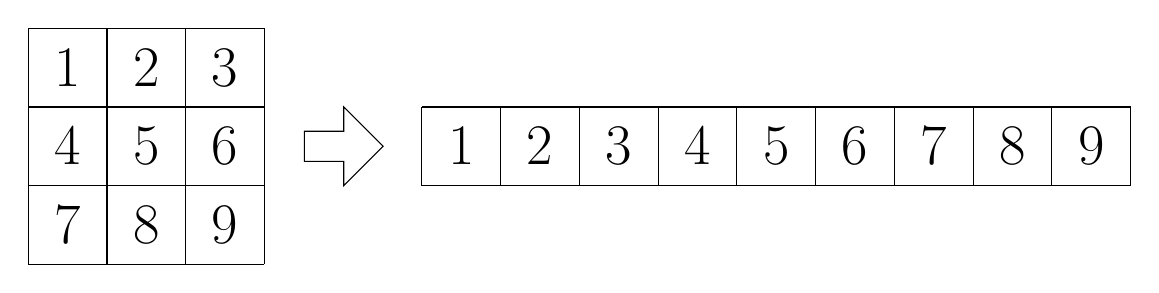
\begin{tikzpicture}
        \usetikzlibrary{shapes.arrows}

        % grid left
        \draw[step=1] (0,0) grid (3,3);
        \node at (.5, 2.5) {\huge 1};
        \node at (1.5, 2.5) {\huge 2};
        \node at (2.5, 2.5) {\huge 3};
        \node at (.5, 1.5) {\huge 4};
        \node at (1.5, 1.5) {\huge 5};
        \node at (2.5, 1.5) {\huge 6};
        \node at (.5, .5) {\huge 7};
        \node at (1.5, .5) {\huge 8};
        \node at (2.5, .5) {\huge 9};

        % arrow
        \node[draw, single arrow,
              minimum height=1cm, minimum width=1cm,
              single arrow head extend=2mm,
              anchor=west] at (3.5,1.5) {};

        % grid right
        \draw[step=1] (5,1) grid (14,2);
        \node at (5.5, 1.5) {\huge 1};
        \node at (6.5, 1.5) {\huge 2};
        \node at (7.5, 1.5) {\huge 3};
        \node at (8.5, 1.5) {\huge 4};
        \node at (9.5, 1.5) {\huge 5};
        \node at (10.5, 1.5) {\huge 6};
        \node at (11.5, 1.5) {\huge 7};
        \node at (12.5, 1.5) {\huge 8};
        \node at (13.5, 1.5) {\huge 9};
    \end{tikzpicture}
    \caption{Flattening, or reshaping, of a 3 by 3 image}\label{fig:flatten}.
\end{figure}
In this section, the pixel space is constructed as a subspace of the 256-dimensional Euclidean space, \(\mathbb{R}^{256}\), which is a Hilbert space~\cite{Bramwell2007}.
This implies that the pixel space is a complete metric space and hence has a valid metric.
Given two vectors, \(\vec{x}\) and \(\vec{y}\), the Euclidean distance~\cite{Bramwell2007} in the pixel space is defined as
\[
    d(\vec{x}, \vec{y}) = \norm{\vec{x} - \vec{y}} = \sqrt{\sum_{i = 1}^{256} {(x_i - y_i)}^2} = \sqrt{(\vec{x} - \vec{y})\cdot (\vec{x} - \vec{y})} = \sqrt{\onenorm{{(\vec{x} - \vec{y})}^{\circ 2}}}.
\]
Here, \(\circ \) denotes the Hadamard power or entrywise power.
The 1-norm, otherwise known as the Taxicab or Manhattan distance, is also a valid metric~\cite{Black2019}.
Given the vectors \(\vec{x}\) and \(\vec{y}\) in the pixel space, the 1-norm distance is defined as
\[ d(\vec{x}, \vec{y}) = \onenorm{\vec{x} - \vec{y}} = \sum_{i = 1}^{256} \abs{x_i - y_i} = \abs{\vec{x}-\vec{y}}.\]
We define \(\vec{x}\) as the image that needs to be classified. Using these metrics, the distances between \(\vec{x}\) and all images of the training set can be calculated.
Then, \(\vec{x}\) is classified as the digit corresponding to the image with the smallest distance to \(\vec{x}\).

The explanation has been abstract thus far, so to make these ideas more concrete a very small example is presented.
For this example, the digit that needs to be classified can be seen in Figure~\ref{fig:test6}. The training set only contains a 4 and a 6, which can be found in Figures~\ref{fig:train6}~and~\ref{fig:train4} respectively.
For convenience, the images in Figures~\ref{fig:test6},~\ref{fig:train6}, and~\ref{fig:train4} will be referred to by the vectors \(\vec{x}, \vec{y}\), and \(\vec{z}\).
\begin{figure}[H]
    \centering
    \begin{subfigure}[b]{.3\textwidth}
        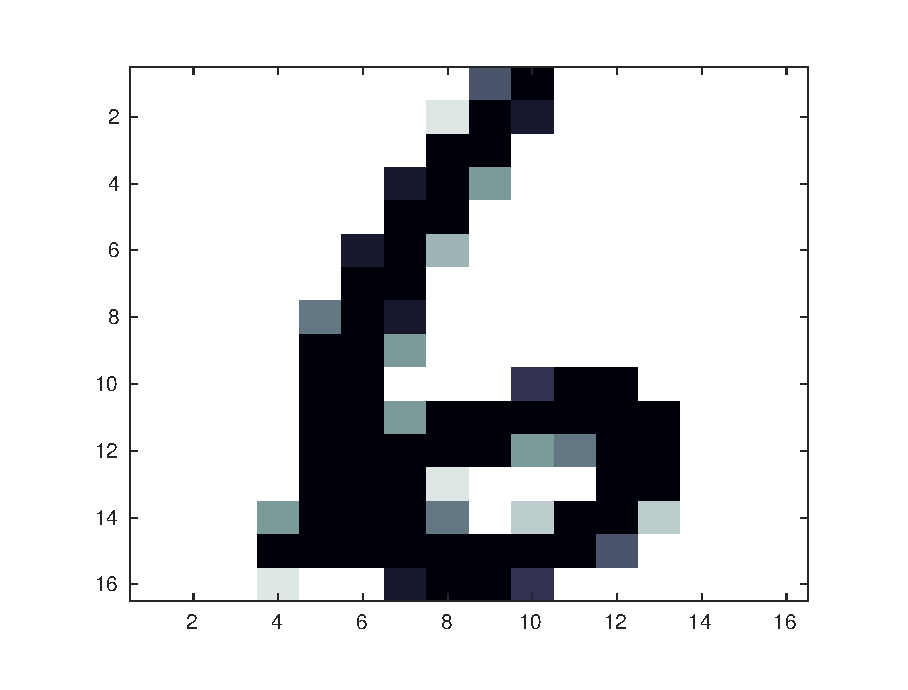
\includegraphics[width = \linewidth]{images/knn/test6.eps}
        \caption{Test digit \(\vec{x}\).}\label{fig:test6}
    \end{subfigure}
    \begin{subfigure}[b]{.3\textwidth}
        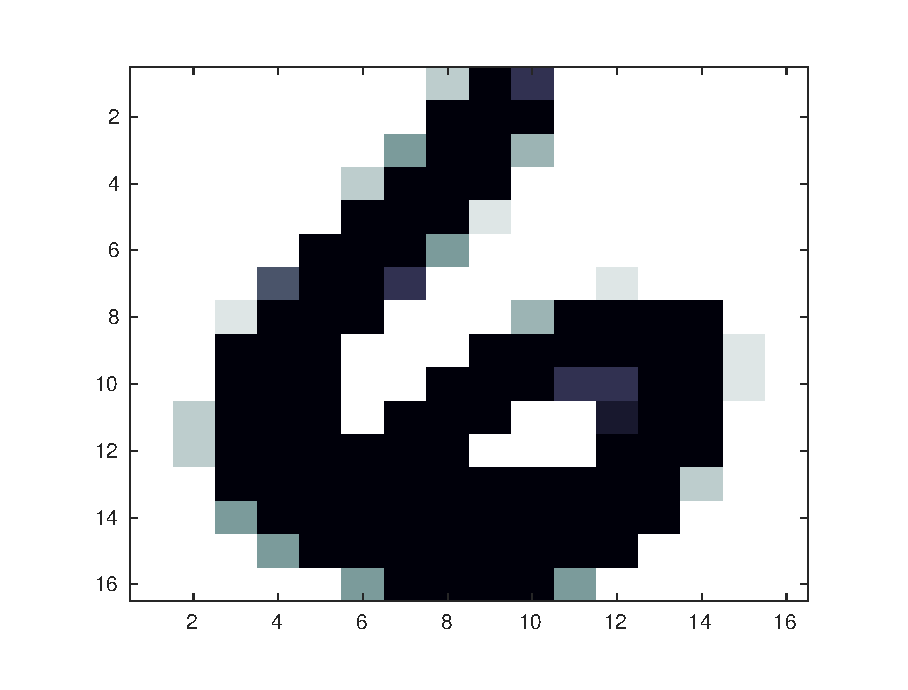
\includegraphics[width = \linewidth]{images/knn/train6.eps}
        \caption{Training data \(\vec{y}\).}\label{fig:train6}
    \end{subfigure}
    \begin{subfigure}[b]{.3\textwidth}
        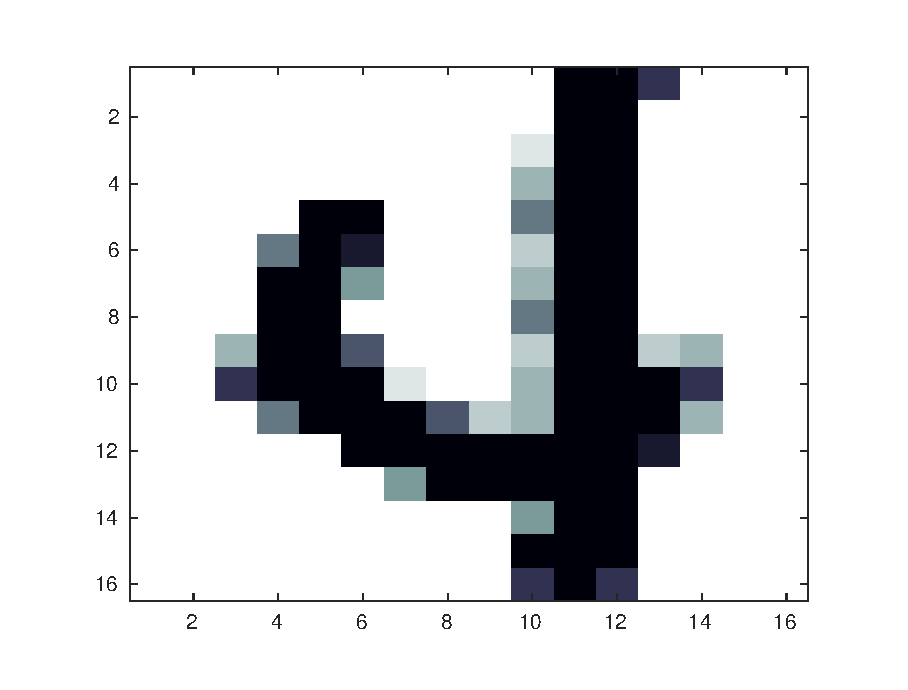
\includegraphics[width = \linewidth]{images/knn/train4.eps}
        \caption{Training data \(\vec{z}\).}\label{fig:train4}
    \end{subfigure}
    \caption{Three different images from the US Postal data set.}
\end{figure}
The first step is to find the distance between \(\vec{x}\) and \(\vec{y}\) and the distance between \(\vec{x}\) and \(\vec{z}\).
In Figures~\ref{fig:difference66}~and~\ref{fig:differenc46} the results of the operations
\[\vec{u} = {(\vec{x} - \vec{y})}^{\circ 2}\text{ and }\vec{v} = {(\vec{x} - \vec{z})}^{\circ 2}\]
can be found.
These operations are the equivalent of taking the pixel wise difference between the two images and then squaring each individual pixel value.
Notice that these operations are present in the definition of the Euclidean distance.
To calculate the distance from this, for both \(\vec{u}\) and \(\vec{v}\) the sum of all the pixel values is taken.
Notice how more overlap between the test and training images lead to ``difference''-vectors with less black values.
\begin{figure}[H]
    \centering
    \begin{minipage}{.3\textwidth}
        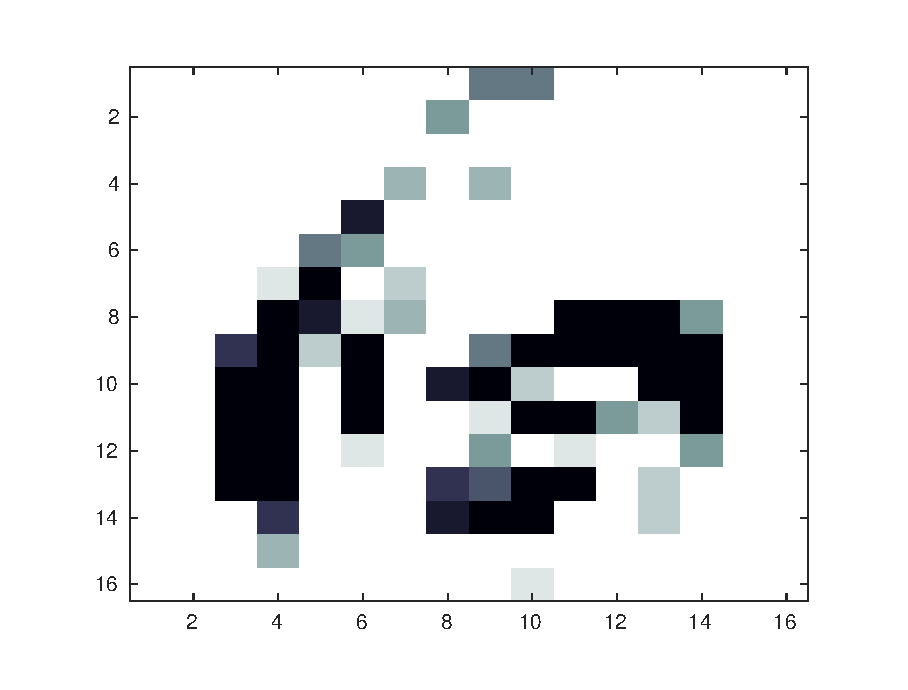
\includegraphics[width = \linewidth]{images/knn/difference66.eps}
        \caption{The vector \(\vec{u}\).}\label{fig:difference66}
    \end{minipage}
    \begin{minipage}{.3\textwidth}
        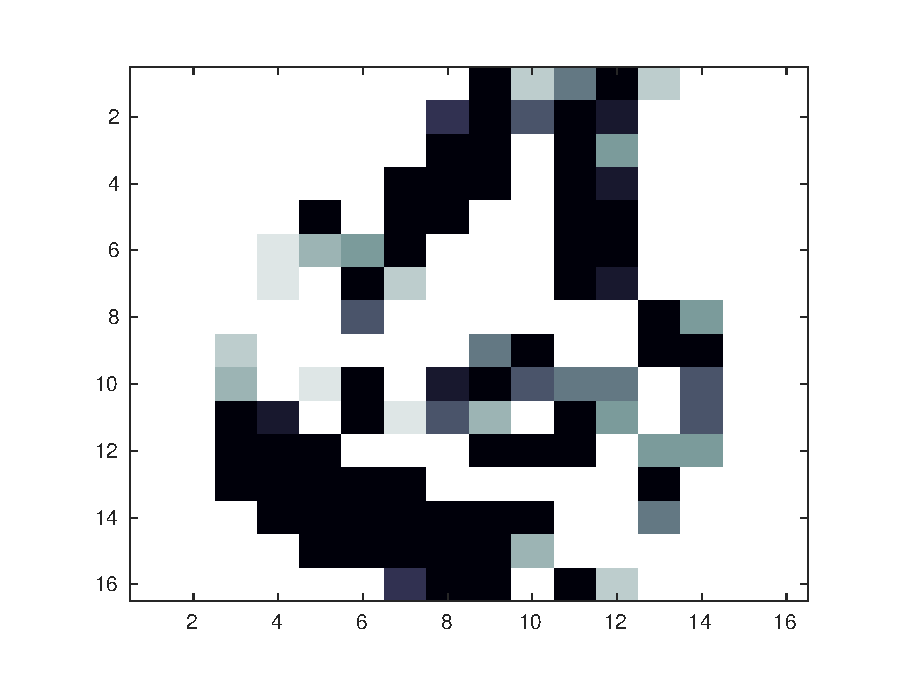
\includegraphics[width = \linewidth]{images/knn/difference46.eps}
        \caption{The vector \(\vec{v}\).}\label{fig:differenc46}
    \end{minipage}
\end{figure}
The sum of all pixel values of \(\vec{u}\) and \(\vec{v}\) are \(12.55\) and \(15.83\).
This means the following:
\begin{align*}
    12.55                                              & < 15.83                                     \\
    \implies \sum_{i = 1}^{256} u_i                    & < \sum_{i = 1}^{256} v_i                    \\
    \implies \sum_{i = 1}^{256} {(x_i - y_i)}^2        & < \sum_{i = 1}^{256} {(x_i - z_i)}^2        \\
    \implies \sqrt{\sum_{i = 1}^{256} {(x_i - y_i)}^2} & < \sqrt{\sum_{i = 1}^{256} {(x_i - z_i)}^2} \\
    \implies \norm{\vec{x} - \vec{y}}                  & < \norm{\vec{x} - \vec{z}}                  \\
    \implies d(\vec{x}, \vec{y})                       & < d(\vec{x}, \vec{z})
\end{align*}
In other words, the result that \(12.55 < 15.83\) implies that \(\vec{x}\) more closely resembles \(\vec{y}\) than \(\vec{z}\).
Since there are only two training samples this also means that the test digit will now be classified as the digit of the most similar image, which is a six.
This is how a digit is classified using the nearest neighbour algorithm in conjunction with the Euclidean distance.

One may note that even though the example was set up to do a correct classification, the difference between \(\vec{u}\) and \(\vec{v}\) is pretty small.
This is related to the fact that the 6 in Figure~\ref{fig:train6} is ``wider'' and ``fatter''.
Furthermore, the Euclidean distance is also susceptible to rotations, scaling and transformations.
The latter of which is illustrated in Figures~\ref{fig:left6}~and~\ref{fig:differenc6left6}.
\begin{figure}[H]
    \centering
    \begin{minipage}{.45\textwidth}
        \centering
        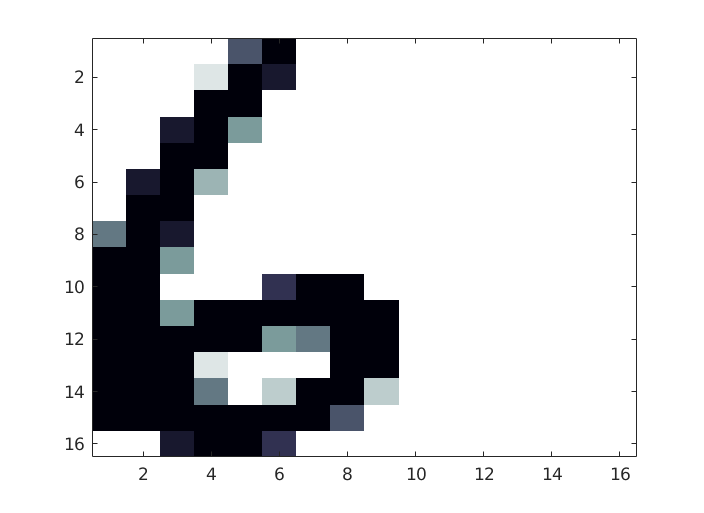
\includegraphics[width = 0.8\linewidth]{images/knn/left6.png}
        \caption{Transposition of \(\vec{x}\).}\label{fig:left6}
    \end{minipage}
    \begin{minipage}{.45\textwidth}
        \centering
        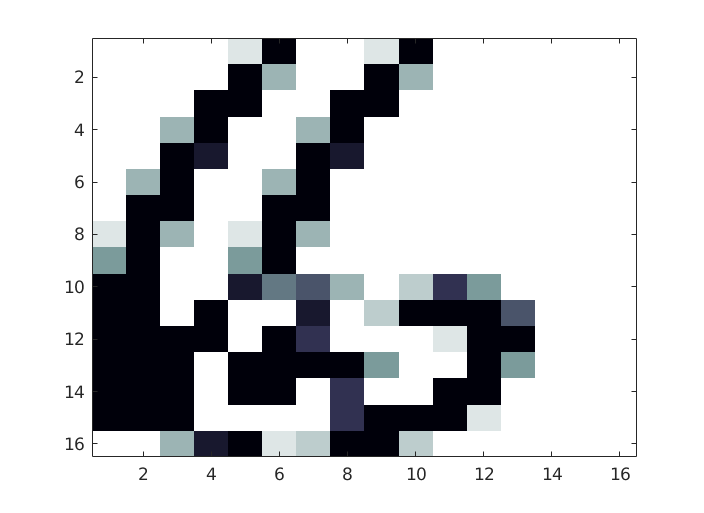
\includegraphics[width = 0.8\linewidth]{images/knn/difference6left6.png}
        \caption{Difference \(\vec{x}\) and its transposition.}\label{fig:differenc6left6}
    \end{minipage}
\end{figure}
The difference between the sum of the elements of Figure~\ref{fig:test6} and the same image shifted left by four pixels is \(17.52\).
This distance is greater than both the other digits.
To deal with these weaknesses the Tangent distance was developed.

\subsubsection{Tangent distance}
As mentioned before, the 1-norm and Euclidean metric are very susceptible to translations and rotations.
The Tangent distance is developed to be invariant with respect to translation, rotation, scaling, shearing, line thickness, and two hyperbolic transforms~\cite{LiweiWang2005}. An example of shearing is the mapping from \((x, y)\) to \((x+2y, y)\).

As we have already established, an image is a point in the 256-dimensional space \(\mathbb{R}^{256}\).
Take a point from this pixel space.
Now, define a transformation.
As example, we take a rotation, such that the parameter corresponds to the angle of the rotation.
Transforming the point according to this rotation yields another point in the pixel space for each angle of rotation.
All points obtained from rotating one point together form a 1-dimensional manifold~\cite{Simard1992, Simard2000}.
It helps to think of this as a line through the pixel space with all slightly rotated versions of the point.
If we take \(P\) to be an image representing a three, then these rotations are the true rotations of \(P\) as can be seen in Figure~\ref{fig:manifold_showcase}.

In case multiple transformations are of interest, the set of transformations can be parametrised by \(n\) parameters. This in turn yields an \(n\)-dimensional manifold.
\begin{figure}[H]
    \centering
    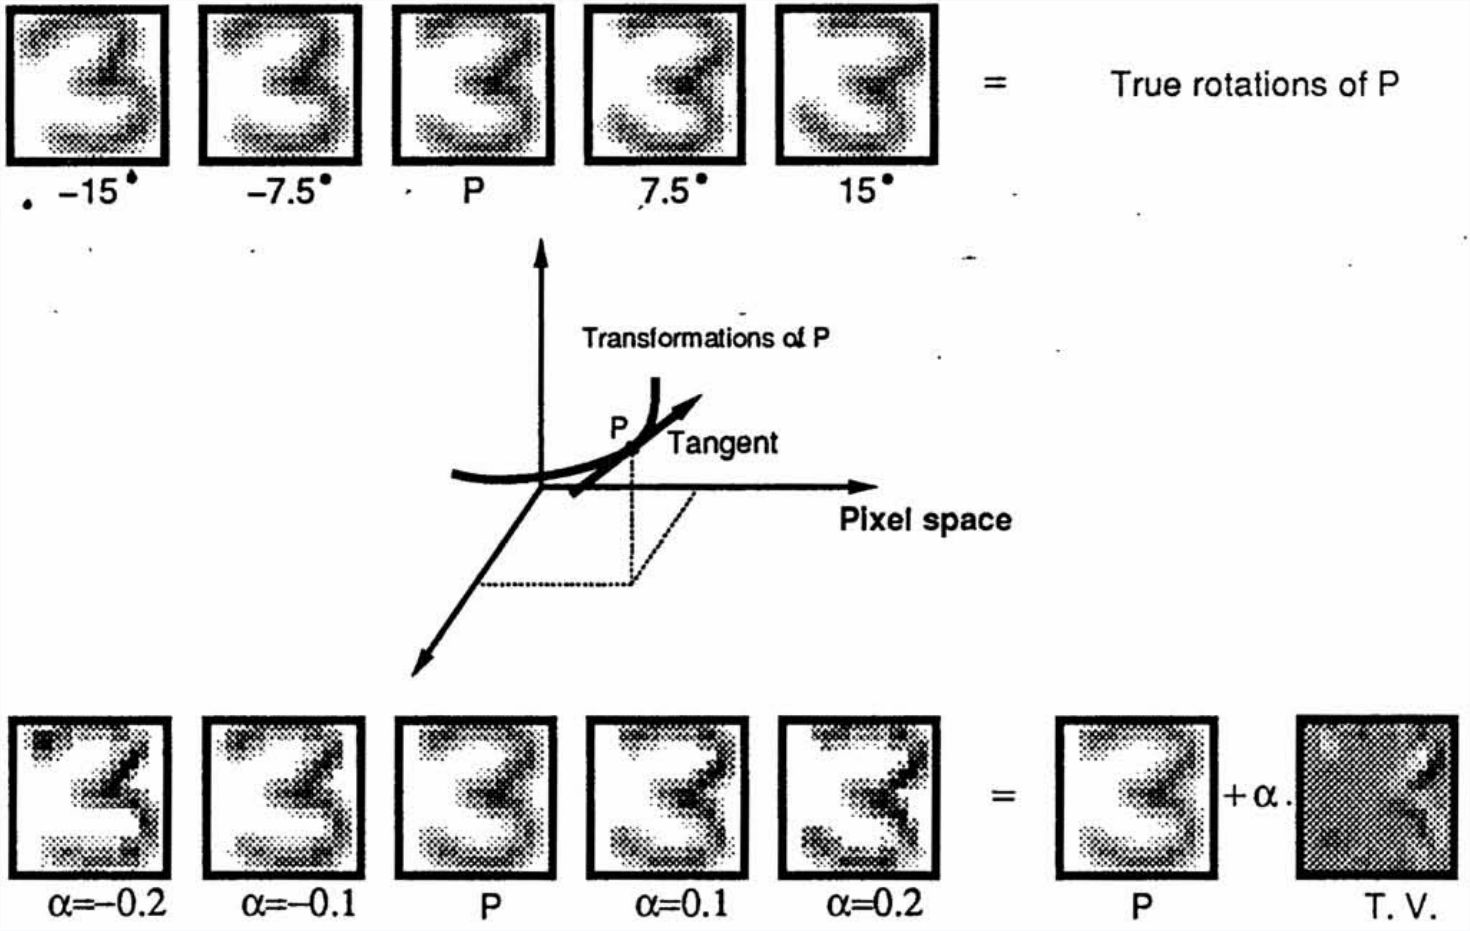
\includegraphics[width = .5\textwidth]{images/knn/manifold_showcase.png}
    \caption{Visual representation of a manifold. Image from Simard et al~\cite{Simard1992}.}\label{fig:manifold_showcase} % background is visible
\end{figure}

The distance between two points can now be defined as the minimum distance between their respective manifolds.
A big problem with this is that the manifold will not be linear, which means that the computation of this distance is a hard non-linear optimization problem~\cite{Keysers2002}.
Alternatively, the distance to the linear approximation of the manifold can be calculated as the approximation is very good for reasonably small angles~\cite{Simard2000}.
The difference can be seen in Figure~\ref{fig:manifold_showcase}, where the resulting rotations of the linear approximation along with tangent vector are shown.
Figure~\ref{fig:manifold_tangent} also shows the difference between the true rotations and the ones created by the linear approximation along with a sketch of the approximation in the pixel space.
Figure~\ref{fig:manifold_distance} visually shows the different distances and how they relate to each other.

\begin{figure}[H]
    \centering
    \begin{minipage}{.45\textwidth}
        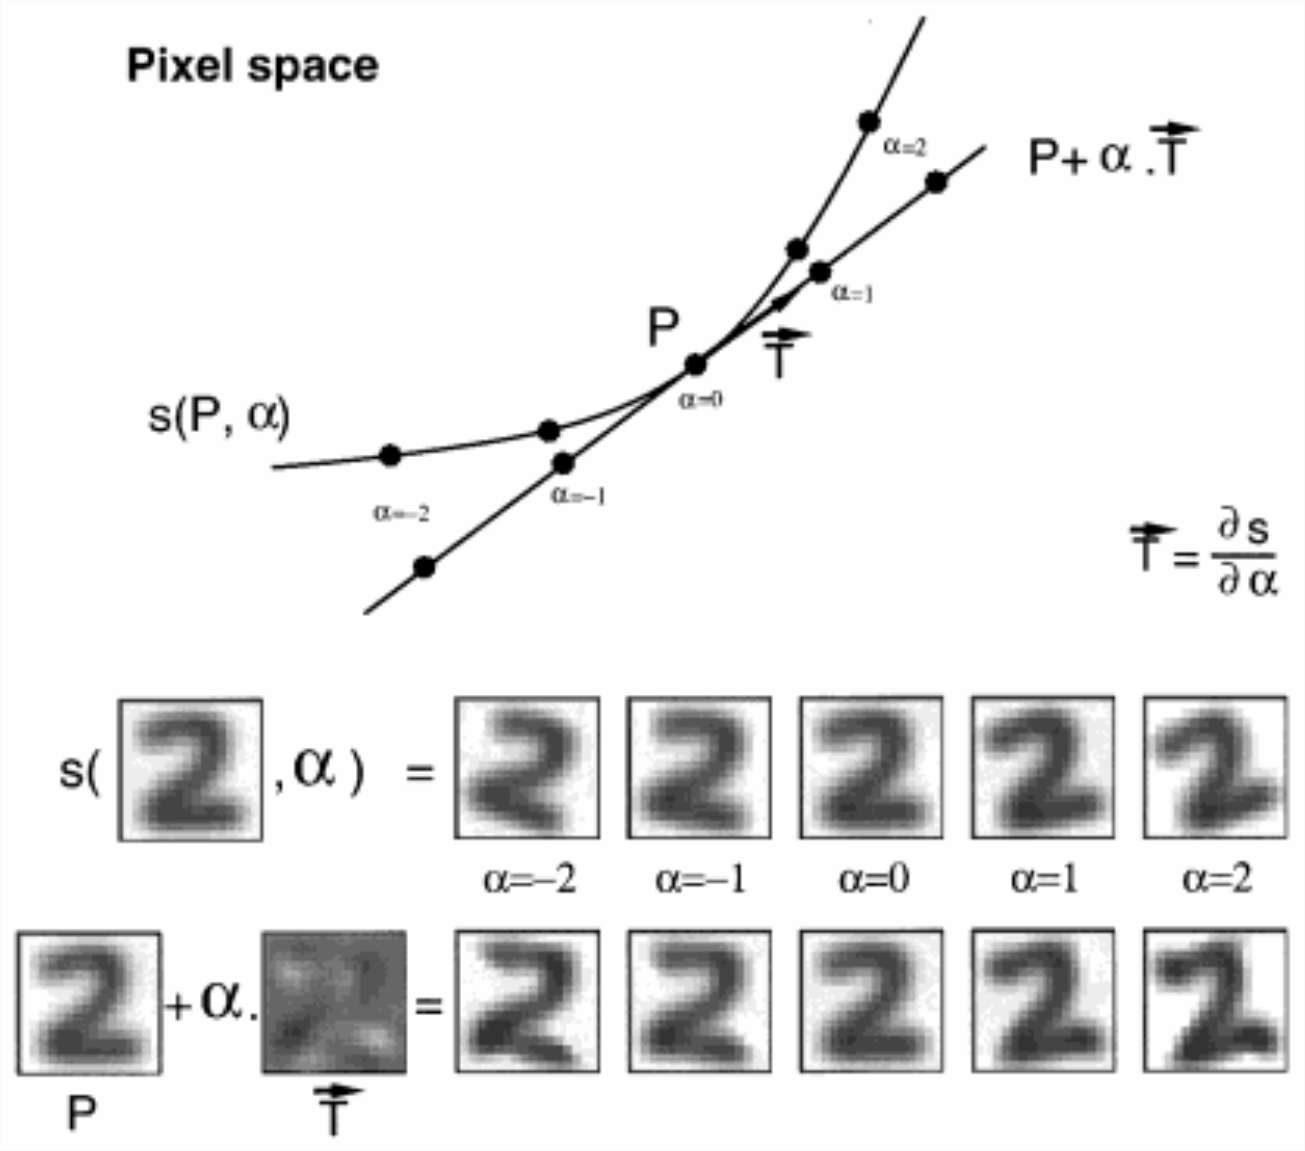
\includegraphics[width = \linewidth]{images/knn/manifold_tangent.png}
        \caption{Tangent of manifold~\cite{Simard2000}.}\label{fig:manifold_tangent}
    \end{minipage}\hspace{1em}
    \begin{minipage}{.45\textwidth}
        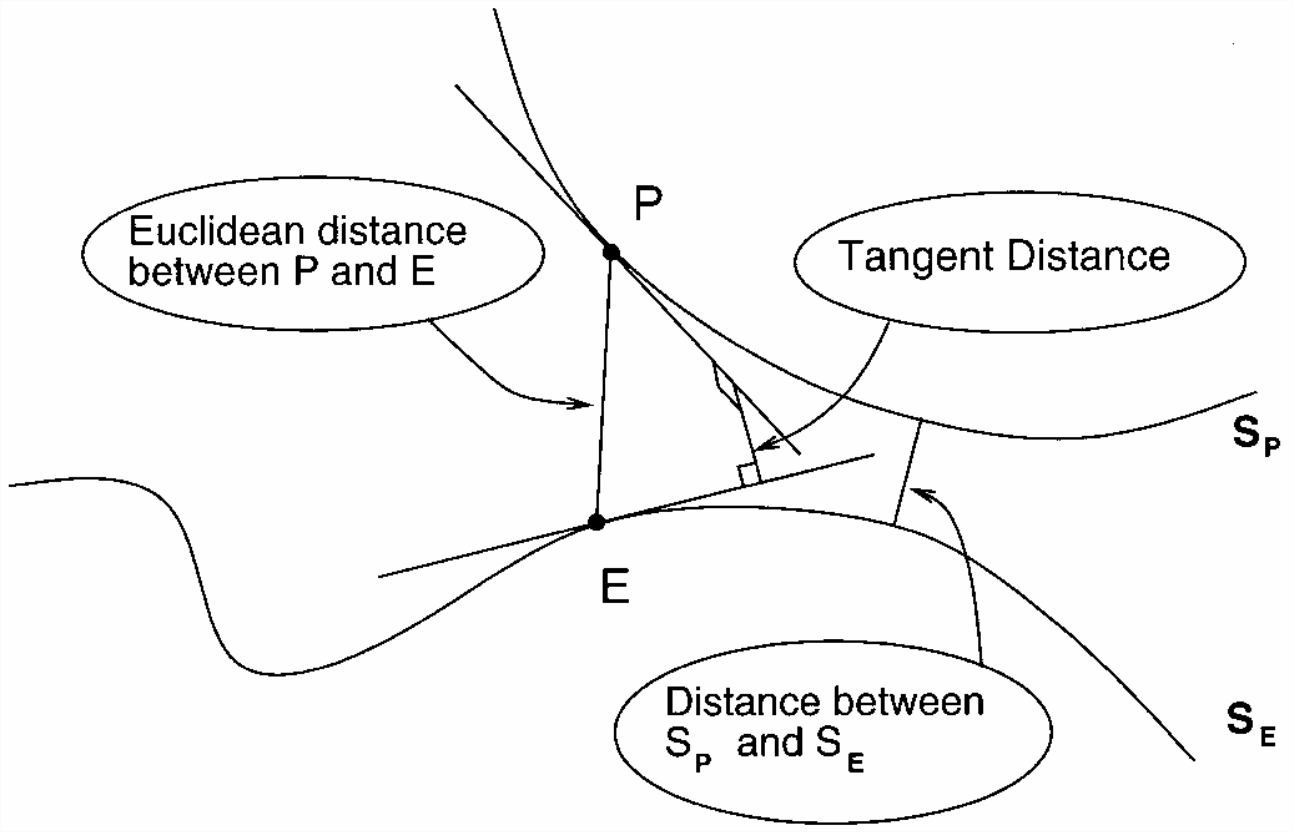
\includegraphics[width = \linewidth]{images/knn/manifold_distance.png}
        \caption{Distances where \(\vec{P}\) and \(\vec{E}\) are points in the pixel space~\cite{Simard2000}.}\label{fig:manifold_distance}
    \end{minipage}
\end{figure}

The main advantage of this approach using the Tangent distance is accuracy as seven chosen transformations mentioned earlier, which should not influence distance, have less impact on the distance compared to Euclidean distance~\cite{LiweiWang2005}.
Naturally, computing the linear approximation results in a lot of computational overhead, increasing the time complexity.
The results which confirm these statements can be found in Table~\ref{tab:knn_all}.

\begin{table}[H]
    \centering
    \caption{Results of nearest neighbour with \(k = 1\).}\label{tab:knn_all}
    \begin{tabular}{l c c c}
        \toprule
        \textbf{Distance} & 1-norm & Euclidean & Tangent \\
        \textbf{Accuracy} & 0.91   & 0.92      & \00.94  \\
        \textbf{Time (s)} & 7.20   & 6.73      & 59.92   \\ \bottomrule
    \end{tabular}
\end{table}
The code to calculate the tangent distance between two images is taken from Keysers et al~\cite{Keysers2002} and was slightly modified to fit the images with a different dimension.

\subsection{Complexity}\label{s:knn:complexity}
Certain applications of digit recognition require a faster classification time than others, such as self-driving cars as compared to writing input on a tablet.
The time complexity describes the amount of time an algorithm takes to run.
All previous subsections discuss the classification of a single digit.
For this single image a distance needs be calculated to every single training image.
This cannot be avoided, however when a second image needs to be classified the distance to each training image should not have to be calculated all over again as the point distribution stays the same.
Certain data structures, such as the \(k\)-d tree, could reduce the amount of distances that need to be calculated.

Besides the computational cost, \(k\)-nearest neighbour as implemented until now is very sensitive to the composition of the training data.
For example, having a lot of sixes compared to zeros will mean that the number six is much more likely to be chosen for a classification.
To solve this, a lot of variations of kNN such as the weighted \(k\)-nearest neighbour, and \(k\)-d tree nearest neighbour have been developed~\cite{Bhatia2010}.

The computational complexity will be derived where useful.

\subsubsection{Linear Search}
The way the classification problem is solved up until this point is with the use of linear search, sometimes called exhaustive or naive search.
It is the ``normal'' implementation of kNN and does not rely on any structuring of the data.
For each image \(\vec{y}\), the distance between \(\vec{y}\) and every other image in the training set is calculated.
The training images are then sorted on their distance to the image \(\vec{y}\).
The most occurring digit in the top \(k\) is picked as the result of the classification.

A tie happens when the two images closest images have different labels.
The case \(k = 2\) results in 293 ties in the used data set, which is \(14.6\% \) of all cases.
The case \(k = 3\) results in no ties happening, which has to do with the fact that a three-way tie is only possible when the three nearest neighbour all represent a different number.
In case of a tie there are several tie-breaking actions that could be chosen:
\begin{itemize}
    \item Choose a different arbitrary \(k\) until there is no longer a tie~\cite{Pylypiw2017}.
    \item Randomly choose between tied values.
          This is the simplest way, however since there is no reason to make a particular a choice. This typically leads to the lowest accuracy~\cite{Pylypiw2017}.
    \item Start with \(k=2\) and increase \(k\) until the tie is broken~\cite{Pylypiw2017}.
    \item Adding weights to the \(k\) values.
          There are several different functions for assigning weights~\cite{Macleod1987}.
          A simple example is \(\frac{1}{d(\vec{x}, \vec{y})}\) as the vector \(\vec{y}\) has the smallest distance to \(\vec{x}\) of the \(k\)-nearest and therefore has the most influence~\cite{Majewski2012}.
          This solution corresponds to the weighted \(k\)-nearest neighbour mentioned earlier~\cite{Bhatia2010}.
\end{itemize}

Now, we reason about the time complexity for linear search.
Let \(t_r\) be the number of training images and \(t_e\) the number of test images.
Since both test and training images have a fixed dimension of \(16 \times 16\), the time complexity of calculating a distance between two images is \(\mathcal{O}(1)\), which is constant.
To classify one image, \(t_r\) number of distances need to be calculated, so the time complexity is \(\mathcal{O}(t_r)\).
To classify \(t_e\) images, the classification of one image is repeated \(t_e\) times, so the total time complexity is \(\mathcal{O}(t_r \cdot t_e)\).

\subsubsection{\textit{k}-d tree}
Calculating the distance between all training images and test images requires a lot of computation, which in turn takes time.
Recall that training images can also be represented by a vector in the Euclidean space and Euclidean space is a vector space in which all points can be ordered with respect to a single dimension.
The idea is to use these properties to create a data structure, such that a lot of candidates can be pruned.
One such data structure is the \(k\)-dimensional tree, or \(k\)-d tree~\cite{Bentley2002}.

The recursive creation of such a \(k\)-d tree with dimensionality \(2\) will be explained.
All entries in the training data set form a set \(S_0\). Sort all the points with respect to their first dimension, here \(x\) coordinates. Now, take the median point as the root node, in the case of Figure~\ref{fig:tree} this is \(A(50, 50)\). Divide all points into two groups, \(S_1\) and \(S_2\), which contain the points with smaller \(x\) coordinates and larger \(x\) coordinates respectively. Now, do this recursively on \(S_1\) and \(S_2\) while using the next dimension, here \(y\) coordinates. Repeat this while cycling through the dimensions until all points are in the \(k\)-d tree.
A \(k\)-d tree can be built in \(\mathcal{O}(kn \log n)\) time~\cite{Brown2015kdtree}.
According to~\cite{Bentley2002}, the asymptotic running time for nearest neighbour queries is empirically observed to be \(\mathcal{O}(\log n)\).

An example of a query is as follows.
Suppose we want to find the nearest point to the point \textbf{Z}\((60, 85)\).
The first coordinate of \textbf{Z} is bigger than \textbf{A}, so in the tree we traverse to the right side.
The second coordinate of \textbf{Z} is bigger than \textbf{C}, so in the tree we traverse to the right side.
The first coordinate of \textbf{Z} is smaller than \textbf{F}, so in the tree we reach a leaf node and \textbf{F} is thus the closest node.
Now, we draw a circle with radius \(d(\textbf{Z}, \textbf{F}) = 10\).
This circle crosses no splitting boundaries, so there cannot be a point closer than \textbf{F}.
In case the circle does cross a splitting boundary, there can be a closer point, so you have to traverse up the tree a check each element in the branch corresponding to the plane the circle crosses.
\begin{figure}[H]
    \centering
    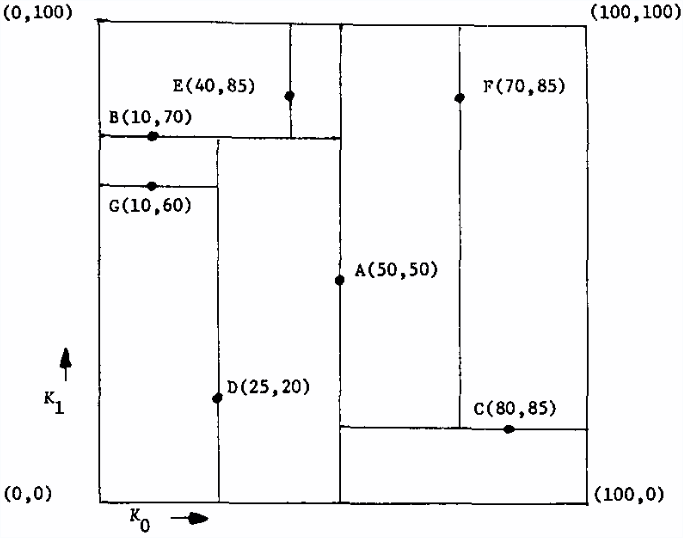
\includegraphics[width = 0.5\textwidth]{images/plane}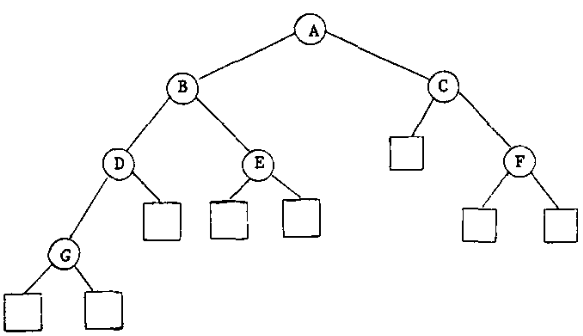
\includegraphics[width = 0.5\textwidth]{images/tree}
    \caption{Points in 2-dimensional space (left) stored as nodes in a 2-d tree (right).}\label{fig:tree}
\end{figure}

\subsubsection{Performance}
The asymptotic running time for nearest neighbour queries of \(\mathcal{O}(\log n)\) only holds for relatively small \(k\), where the logarithmic behaviour is observed on a large number of training samples.
Due to the sparsity of the data, for large \(k\) this effect becomes even more pronounced.
For example, for \(k = 16\) a search of a \(k\)-dimensional tree of 76,000 records examines almost every record, which means that (almost) no pruning is happening and that the tree has lost its purpose~\cite{Sproull1991}.
To put this into perspective, the data set in this paper has a dimensionality of \(k = 256\) with only 1,707 training images.
As a result, using the \(k\)-d tree still requires that the distance to all training images needs to be calculated to find the most similar one, while incurring the overhead of precomputing the data structure.
This can be seen in the results in Table~\ref{tab:knn_anthon}.
Since the \(k\)-d tree nearest neighbours queries take as much time as the linear search, the estimated data structure overhead is as much as \(25\% \).
\begin{table}[H]
    \centering
    \caption{Results of kNN on training data set. The time includes preprocessing and the querying of all test images.}\label{tab:knn_anthon}
    \begin{tabular}{l c c c c c}
        \toprule
        \textbf{\(k\)}             & 1    & 2    & 3    & 4    & 5    \\
        \textbf{Accuracy}          & 0.92 & 0.90 & 0.91 & 0.90 & 0.90 \\
        \textbf{Time Linear (s)}   & 0.34 & 0.30 & 0.31 & 0.29 & 0.30 \\
        \textbf{Time k-d tree (s)} & 0.59 & 0.36 & 0.34 & 0.36 & 0.37 \\ \bottomrule
    \end{tabular}
\end{table}
Furthermore, unexpectedly the accuracy only decreases as \(k\) increases.
This can be explained as a combination of sparse data and no labelling errors in the training set.
A consequence of the sparsity of the data is that images with a bigger distance to the unknown image are included and exercise influence on the classification of that image. Paraphrased, this means that more and more irrelevant images are used to classify an image, hence leading to less accurate results.

Note that the times are not comparable with Table~\ref{tab:knn_all}.
This is related to the fact that the algorithm was run on an implementation which is specifically crafted to only be influenced by the time the distance calculation takes without any other optimizations such as to have a level playing field.

\subsection{Approximate methods}\label{s:knn:approximate}
Storing the data in \(k\)-d trees did not prove successful in bringing down the running time for applications with a time constraint.
For these kinds of applications, derivatives of the \(k\)-nearest neighbour method have been developed under the name approximate nearest neighbour.

This class of nearest neighbour techniques exploits redundancy to reduce the computational cost.
The training data set in this paper has 1,707 entries, which contains 252 images representing the number one.
There is guaranteed to be a lot of overlap between these images.
The name contains ``approximate'', because reducing overlap almost always comes in some form of data simplification where some information will be lost.

The term approximate nearest neighbours is a hypernym, meaning that there are many algorithms falling under the name such as locality sensitive hashing, clustering, etcetera~\cite{Rajaraman2011, Bhatia2010}.
Ultimately, approximate nearest neighbour only yields improvement in time complexity and memory use, while sacrificing some accuracy.

\subsubsection{Nearest Mean}
One way to reduce redundancy and overlap is by grouping together duplicate images. All metrics have the properties and results for vectors such that \(\vec{x} = \vec{y}\):
\begin{align*}
    \vec{x}                      & = \vec{y} \implies d(\vec{x}, \vec{y}) = 0                           & \text{See~\cite{Simard1992,Bramwell2007}} \\
    d(\vec{x}, \vec{z})          & \leq d(\vec{x}, \vec{y}) + d(\vec{y}, \vec{z}) = d(\vec{y}, \vec{z})                                             \\
    d(\vec{y}, \vec{z})          & \leq d(\vec{y}, \vec{x}) + d(\vec{x}, \vec{z}) = d(\vec{x}, \vec{z})                                             \\
    \implies d(\vec{x}, \vec{z}) & = d(\vec{y}, \vec{z})
\end{align*}
This proves that the distance from an arbitrary image to two identical training images will be the same.
This means that duplicates in the training data set can be removed without affecting the accuracy of the algorithm.

The sparsity of the data implies that the amount of duplicates in the training set will be very limited, hence this will barely improve the speed.
If more performance is still desired, images with very small differences can then be merged.
The threshold for clustering two images has to be experimented with to find the optimal value.
However, this is a trade-off, since a lower threshold will yield better accuracy, yet a lower performance and vice versa.
Setting the threshold to 0 will give the same results as the ``standard'' nearest neighbours, while setting no bound for the threshold will result in merging everything and yield the nearest mean.

With no bound, all images of the same class are merged into a vector.
This vector will simply be the average image for each class.
On the left side in Figure~\ref{fig:train_3} a normal 3 can be seen beside the ``average'' 3.
Here, the loss of information is also clearly illustrated.
\begin{figure}[H]
    \centering
    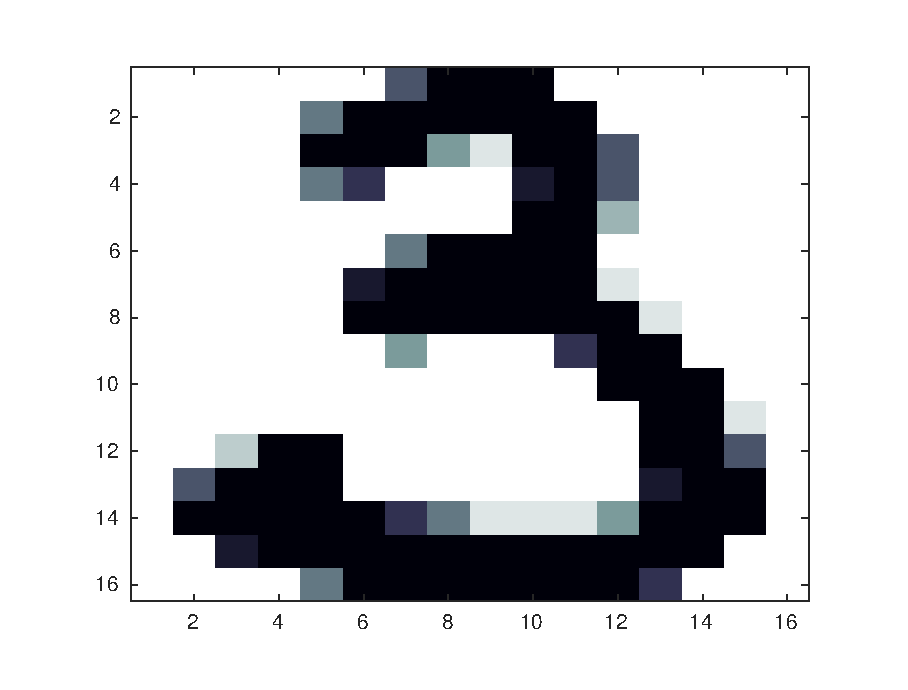
\includegraphics[width = 0.3 \textwidth]{images/train_3.eps}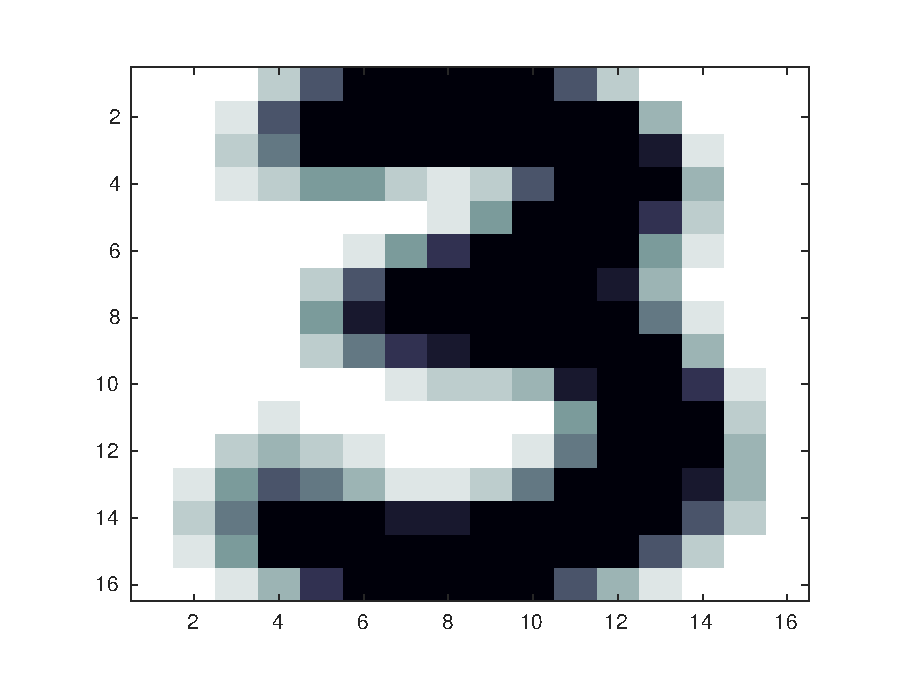
\includegraphics[width = 0.3 \textwidth]{images/average_3.eps}
    \caption{A 3 occurring in the training set and the average 3 vector.}\label{fig:train_3}
\end{figure}
As stated before, the computation of all of the mean images takes \(\mathcal{O}(t_r)\) time, with \(t_r\) the number of training images.
The main advantage of this approach is speed, since each test image has to be checked against only 10 other images.
As a result, a single classification has a time complexity of \(\mathcal{O}(1)\) for an image of a fixed size.
For \(t_e\) number of classifications the total asymptotic computational complexity is \(\mathcal{O}(t_e + t_r)\).

The results, as seen in Table~\ref{tab:mean_anthon}, portray a significant speed advantage over the results seen in Table~\ref{tab:knn_all}.
An important thing to note is that each class now only has one representative.
As a result, the linear approximations of the manifolds cannot overlap with images already present in the training set.
This in turn leads to the Tangent distance yielding a much bigger improvement over the Euclidean distance, while having relatively the same performance penalty.

\begin{table}[H]
    \centering
    \caption{Results of Nearest Mean.}\label{tab:mean_anthon}
    \begin{tabular}{l c c c}
        \toprule
        \textbf{Distance} & 1-norm & Euclidean & Tangent \\
        \textbf{Accuracy} & 0.71   & 0.81      & 0.88    \\
        \textbf{Time (s)} & 0.04   & 0.03      & 0.34    \\
        \bottomrule
    \end{tabular}
\end{table}
Note that the Tangent distance in these tests is implemented in C compiled with Mex, so the time values of the Tangent distance can only be meaningfully compared with the same implementations in this paper.

In this section the distance from a new image to (a subset of) all images in the training set was used to identify images.
The images associated with the same number span a subspace of \(\mathbb{R}^{256}\).
In the next section the distance to this subspace will be used to classify digits instead.